%%%%%%%%%%%%%%%%%%%%%%%%%%%%%%%%%%%%%%%%%%%%%%%
%%%     Declarations (skip to Begin Document, line 88, for parts you fill in)
%%%%%%%%%%%%%%%%%%%%%%%%%%%%%%%%%%%%%%%%%%%%%%%

%%\documentclass[10pt]{article}
%%\documentclass[10pt]{report}
\documentclass[letterpaper]{article}
\usepackage{geometry}
%\usepackage{xcolor}
\usepackage[table]{xcolor}
\usepackage{amsmath}
\usepackage[some]{background}
%\usepackage{lipsum}
%\usepackage{natbib}
\usepackage{siunitx}

% C I T A T I O N S
\usepackage[backend=biber, style=apa]{biblatex}  
%\usepackage{biblatex} 
\addbibresource{paperpile.bib}

\usepackage[hidelinks]{hyperref}

% C A P T I O N S
%\usepackage{caption, copyrightbox}
%\captionsetup{justification=centering, labelfont=sc, labelsep=endash}

% Tables
\usepackage{float}
\usepackage[utf8]{inputenc}
\usepackage{tabularx}
\usepackage{booktabs}
\usepackage{longtable}

\usepackage{diagbox} %table split headers
\usepackage{longtable}
\usepackage{array}
\usepackage{rotating}
\usepackage{eqparbox}
\usepackage{makecell, caption, booktabs}

% Stuff needed to get table to span pages
\usepackage{enumitem}
%\usepackage{array, booktabs, longtable}
\newcolumntype{x}[1]{>{\raggedright}p{#1}}

\usepackage{etoolbox}
\AtBeginEnvironment{longtable}{%
    \setlist[itemize]{nosep,     % <-- new list setup
                      topsep     = 0pt       ,
                      partopsep  = 0pt       ,
                      leftmargin = *         ,
                      label      = $\bullet$ ,
                      before     = \vspace{-\baselineskip},
                      after      = \vspace{-0.5\baselineskip}
                        }
                           }% end of AtBeginEnvironment
% End table span
% Listings
\usepackage{listings}

\usepackage{geometry}  % Lots of layout options.  See http://en.wikibooks.org/wiki/LaTeX/Page_Layout
\geometry{letterpaper}  % ... or a4paper or a5paper or ... 
\usepackage{fullpage}  % somewhat standardized smaller margins (around an inch)
\usepackage{setspace}  % control line spacing in latex documents
\usepackage[parfill]{parskip}  % Activate to begin paragraphs with an empty line rather than an indent

\usepackage{amsmath,amssymb}  % latex math
\usepackage{empheq} % http://www.ctan.org/pkg/empheq
\usepackage{bm,upgreek}  % allows you to write bold greek letters (upper & lower case)

% for typsetting algorithm pseudocode see http://en.wikibooks.org/wiki/LaTeX/Algorithms_and_Pseudocode
\usepackage{algorithmic,algorithm}  

\usepackage{graphicx}  % inclusion of graphics; see: http://en.wikibooks.org/wiki/LaTeX/Importing_Graphics
% allow easy inclusion of .tif, .png graphics
\DeclareGraphicsRule{.tif}{png}{.png}{`convert #1 `dirname #1`/`basename #1 .tif`.png}

% \usepackage{subfigure}  % allows subfigures in figure
\usepackage{caption}
\usepackage{subcaption}

\usepackage{xspace}
\newcommand{\latex}{\LaTeX\xspace}

\usepackage{color}  % http://en.wikibooks.org/wiki/LaTeX/Colors

\long\def\todo#1{{\color{red}{\bf TODO: #1}}}

\long\def\ans#1{{\color{blue}{\em #1}}}
\long\def\ansnem#1{{\color{blue}#1}}
\long\def\boldred#1{{\color{red}{\bf #1}}}
\long\def\boldred#1{\textcolor{red}{\bf #1}}
\long\def\boldblue#1{\textcolor{blue}{\bf #1}}

% Useful package for syntax highlighting of specific code (such as python) -- see below
\usepackage{listings}  % http://en.wikibooks.org/wiki/LaTeX/Packages/Listings
\usepackage{textcomp}


%%% The following lines set up using the listings package
\renewcommand{\lstlistlistingname}{Code Listings}
\renewcommand{\lstlistingname}{Code Listing}

%%% Specific for python listings
\definecolor{gray}{gray}{0.5}
\definecolor{green}{rgb}{0,0.5,0}

\lstnewenvironment{python}[1][]{
\lstset{
language=python,
basicstyle=\footnotesize,  % could also use this -- a little larger \ttfamily\small\setstretch{1},
stringstyle=\color{red},
showstringspaces=false,
alsoletter={1234567890},
otherkeywords={\ , \}, \{},
keywordstyle=\color{blue},
emph={access,and,break,class,continue,def,del,elif ,else,%
except,exec,finally,for,from,global,if,import,in,i s,%
lambda,not,or,pass,print,raise,return,try,while},
emphstyle=\color{black}\bfseries,
emph={[2]True, False, None, self},
emphstyle=[2]\color{green},
emph={[3]from, import, as},
emphstyle=[3]\color{blue},
upquote=true,
morecomment=[s]{"""}{"""},
commentstyle=\color{gray}\slshape,
emph={[4]1, 2, 3, 4, 5, 6, 7, 8, 9, 0},
emphstyle=[4]\color{blue},
literate=*{:}{{\textcolor{blue}:}}{1}%
{=}{{\textcolor{blue}=}}{1}%
{-}{{\textcolor{blue}-}}{1}%
{+}{{\textcolor{blue}+}}{1}%
{*}{{\textcolor{blue}*}}{1}%
{!}{{\textcolor{blue}!}}{1}%
{(}{{\textcolor{blue}(}}{1}%
{)}{{\textcolor{blue})}}{1}%
{[}{{\textcolor{blue}[}}{1}%
{]}{{\textcolor{blue}]}}{1}%
{<}{{\textcolor{blue}<}}{1}%
{>}{{\textcolor{blue}>}}{1},%
%framexleftmargin=1mm, framextopmargin=1mm, frame=shadowbox, rulesepcolor=\color{blue},#1
framexleftmargin=1mm, framextopmargin=1mm, frame=single,#1
}}{}
%%% End python code listing definitions

\DeclareMathOperator{\diag}{diag}
\DeclareMathOperator{\cov}{cov}


%\bibliography{./paperpile.bib}
\author{Evan McGinnis}
\title{Automated Weeding}



\definecolor{titlepagecolor}{cmyk}{1,.60,0,.40}

\DeclareFixedFont{\bigsf}{T1}{phv}{b}{n}{1.5cm}

\backgroundsetup{
scale=1,
angle=0,
opacity=1,
contents={\begin{tikzpicture}[remember picture,overlay]
 \path [fill=titlepagecolor] (-0.5\paperwidth,5) rectangle (0.5\paperwidth,10);  
\end{tikzpicture}}
}
\makeatletter                       
\def\printauthor{%                  
    {\large \@author}}              
\makeatother
\author{%
    Evan McGinnis \\
    Graduate Student \\
    Biosystems Analytics \\
    \texttt{evanmc@arizona.edu}\vspace{40pt} \\
    }
\begin{document}
\begin{titlepage}
\BgThispage
\newgeometry{left=1cm,right=4cm}
\vspace*{1cm}
\noindent
%%\vspace*{0.4\textheight}
\textcolor{white}{\Huge\textbf{\begin{flushleft}\textsf{Imbalanced Learning in\linebreak Crop/Weed Classification}\end{flushleft}}}
\vspace*{3.5cm}\par
\noindent
\begin{minipage}{0.35\linewidth}
    \begin{flushright}
        \printauthor
    \end{flushright}
\end{minipage} \hspace{15pt}
%
\begin{minipage}{0.02\linewidth}
    \rule{1pt}{175pt}
\end{minipage} \hspace{-10pt}
%
\begin{minipage}{0.70\linewidth}
\vspace{5pt}
    \begin{abstract} 
This paper presents an overview of solutions to an all to common problem in the classification of vegetation in agricultural images: there are many more crop plants than there are weeds. The solution examined is the generation of synthetic data.
    \end{abstract}
\end{minipage}
\end{titlepage}
\restoregeometry
%
% F R O N T  M A T T E R
%
\tableofcontents
\listoffigures
\listoftables
%\listofequations
\newpage

%` 
% O V E R V I E W 
%



\section{Introduction}
Agricultural images of crops taken from an overhead perspective typically contain only two things: crop and weeds. While images taken from more than a meter AGL sometimes contain infrastructure equipment, and there may be other non-vegetative debris on the ground, crop and weed plants are the concern here. The application of a vegetation index to the image typically eliminates all non-vegetated elements of an images, leaving only the aforementioned plants. Fortunately for the grower, but unfortunately for classification, these images often contain a much higher portion of crop than they do weeds, particularly if a pre-emergent herbicide has been applied or other active weed control measures are taken (TODO: Citation) Having 10 weeds out of 100 plants in an image set might not be much of a problem, but having only three might be, especially taking into account a train/test split. The result may be that a weed is represented by only one or two samples.

\section{Methodology}
Images were taken at the University of Arizona's Maricopa Agricultural Center (MAC) located in Maricopa, AZ of a cantaloupe planting in May 2024 (N 33.061813 W 111.965606). Images were obtained using an Apple iPhone 14, using ambient lighting. These images were color corrected using values obtained from images taken under identical lighting conditions of a Datacolor Spyder correction chart using Adobe Lightroom.  Images obtained using other sources are used to illustrate techniques or points, but most of the analysis shown in this document are from the set gathered at the MAC. All processing software was written in Python 3 and data analysis written in R.  The processing software depended heavily on three libraries: OpenCV (image processing), imbalanced-learn (imbalance correction), and scikit-learn (machine learning). The image sets examined were segmented using the Combined Indices 2 approach described by \citeauthor{Guerrero2012-zi} and manually assigned classification \parencite{Guerrero2012-zi}.
Present in the image sets are two types of vegetation: crop and weeds. While the ratio of crop to weeds will most assuredly deviate from the 1:1 ideal, it is not particularly important what the specific ratio is, as the data will be trimmed to reflect the various ratios. That is, while a dataset may have a relatively low imbalance of 10:8, samples of the minority class are randomly discarded to achieve a much higher imbalance, say 50:1. Not covered in this breakdown, but quite important, is the topics of when to use imbalance correction techniques and when to perform parameter selection. This analysis will use a fairly commonly used train/test split of the data to form, and then test models. It is on this train set that the imbalance is corrected -- the objective is not to classify samples that are the result of correction, but to build a model that will produce results that exceed doing no correction. Parameter selection has similar concerns, but has some complications that merit mention here. Each plant in the image has color, texture, and shape attributes that are extracted and then the subset identified by PCA is used. The details of the extracted parameters is beyond the scope of this document, but what is not is when the parameter analysis takes place. Parameter analysis takes place prior to any imbalance correction.  As section \ref{section:over} details, new, synthetic entries can be constructed as part of imbalance correction, but the corrections are not considered in parameter selection, just the original data.

\section{Class Imbalance}
Plantings often exhibit a somewhat inconvenient feature: weeds and crop do not appear in the same proportion. While having a low weed count is probably desirable for crop production, it is not for classification when considering those images as a training set. While this can present itself as a relatively mild imbalance of nine weed plants for every 10 crop plants or a more extreme ratio of 1000 crop plants for every weed. In these extreme cases of imbalance, only a few samples of the minority class are used in classification if the overall size of the population is not particularly large -- and even more unfortunate case is that some weed species may not be present at all in the set used for training, as they are put into a testing class. \citeauthor{Fernandez2018-fw}, in a book discussing imbalanced datasets, detail several correction algorithms, among them SMOTE, ADASYN, Borderline SMOTE, kmeans, and SVM \parencite{Fernandez2018-fw}. These algorithms seek to address the imbalance by the creation of synthetic samples of the minority class, correcting the class ratio to 1:1.  In most cases. of course, the solution is to simply collect sufficient data such that a severe imbalance does not exist, but this may not be a practical solution. This leaves two approaches: under-sample the majority or over-sample the minority. In cases where weeds (the minority) are relatively few, providing synthetic data to restore data to a 1:1 class ratio may be effective. There are various approaches that all have the same basic approach: generate data from the minority class that is similar -- but not identical -- to the data already present. That is, the minority class is over-sampled.  Alternatively, the majority class can be under-sampled to achieve a 1:1 ratio, typically in two ways: randomly, and mathematical techniques that are more sensitive to the data relationships in the majority class.

\section{Over-Sampling}
\label{section:over}
Over-sampling is a bit more complex than the term implies -- minority samples are not simply sampled until the numbers are equal to a majority class. Just duplicating entries can correct the imbalance ratio back to the more desired 1:1, but does not add new data to the models being built than can be used to classify novel instances. Rather, new samples of the minority class are created, but the key question is \textit{which} of those minority instances form the basis of those synthetic samples? Are they chosen at random? Are they selected somehow?  This question of which sample points in the minority set are used will be a topic revisited often as various techniques are described, as what points are used.

 
\subsection{SMOTE}
The \textit{Synthetic Minority Oversampling TEchnique} is the basic technique used for re-balancing the data set -- other techniques in this section are extensions to that approach \parencite{Chawla2002-dk}. Synthetic data is generated by selecting examples that are close in terms of the \textit{k} nearest neighbors, and selecting new points along the line connected those peers.
\begin{figure}[H]
	\centering
	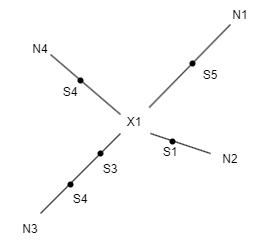
\includegraphics[scale=0.35]{./figures/smote.png}
	\caption[SMOTE selection of synthetic data points]{Generating synthetic data points using the SMOTE algorithm considers the \textit{k} nearest neighbors ($N_{1..4}$) to a point under consideration ($X_1$).  The SMOTE algorithm identifies points along the lines connecting a point to its neighbors ($S_{1..5}$). These points are the synthetic samples used to correct the imbalance.}
	\label{fig:smote}
\end{figure}

\subsection{ADASYN}
The Adaptive Synthetic Sampling approach considers the distribution of the minority points, giving more emphasis to points that a harder to learn. \parencite{He2008-xr} Points that are harder to learn are those that are close to a class border, and in that sense, this approach is close to the \text{borderline} proposal. Contrast this with SMOTE. While sharing the same basic approach (considering the $k$ nearest neighbors), SMOTE samples the points uniformly, leading to an oversampling of dense areas, whereas ADASYN has no fixed ratio, but is based on learning difficulty. ADASYN will generate more points for these samples with high learning when processing the same dataset. The term \textit{harder to learn} is a bit imprecise, and warrants some further discussion. ADASYN creates as difficulty ratio for each point, representing the imbalance level in the local neighborhood of the point. This is done by comparing the number of majority class instances (non-minority) to the number of minority class instances within a specified radius around a point. Minority points with a large set of majority class neighbors are said to be harder to learn than those.


\subsection{Borderline}
In the standard SMOTE approach all members of the minority class are considered in synthetic data generation. In this variant first proposed by \citeauthor{Han2005-ui}, only those points far from the class border are considered. The rationale behind this approach is that points close to the border contribute little to distinguishing one class from the other, and should not form the basis for new data \parencite{Han2005-ui}. In this scheme, points are considered noise if all of their neighbors are of the majority class. To be eligible for resampling, however, a point must have both majority and minority class neighbors. The rationale here is that samples close to a class border tend to be misclassified, and that by limiting the resampling to those points with the smallest risk of misclassification, the overall correct classification rate would be improved.
\begin{figure}[H]
	\centering
	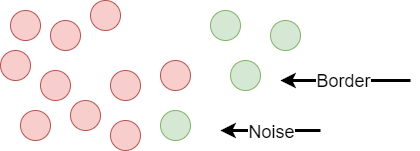
\includegraphics[scale=0.30]{./figures/borderline.png}
	\caption[Borderline selection of synthetic data points]{In the borderline variant of SMOTE, points close to the border having only majority class neighbors are considered noise, and are not considered as candidates for selection.}
	\label{fig:borderline}
\end{figure}



\subsection{KMeans}
This variant, like many of the others described here, addresses a weakness in basic SMOTE: points are selected randomly for oversampling consideration. A further downside of the base algorithm is the noise it introduces. This is not so much a SMOTE variant as it is a SMOTE supplement. As \citeauthor{Last2017-rh} states in a document introducing the algorithm:
\begin{quote}
\textit{
Another major concern is that SMOTE may further amplify noise present in the data. This is likely
to happen when linearly interpolating a noisy minority sample, which is located among majority class
instances, and its nearest minority neighbor. \parencite{Last2017-rh}
}
\end{quote}
This approach differs from algorithms such as \textit{borderline} in that this approach views the class to be adjusted in terms of cluster membership.  In this approach, the clusters are formed with the \textit{kmeans} approach and SMOTE is applied to those clusters with a high portion of the minority class.

%
% This article seems to be available only for purchase as the library does not subscribe to that journal
% This is the reference both for borderline and SVM
%
\subsection{Support Vector Machine}
SVM SMOTE increases the points for the minority class along the decision boundary by generating new points along the lines connecting the support vectors and nearest neighbors \parencite{Nguyen2011-cb}. In contrast with the KMeans approach, but in the same spirit as the borderline approach, this approach considers those points more important for estimating the best decision boundary, and therefor the best candidates for synthetic data generation.

\subsection{Assessing Techniques}
To assess the efficacy of the creation of synthetic data, instances in a dataset were first dropped to achieve five imbalance ratios and then restored to a 1:1 ratio between the two classes using the over-sampling techniques discussed. Models using the imbalanced data and the artificially balanced data were then compared in terms of the improvement (or degradation) of the F1 score using nine different techniques (Random Forest, Extra Trees, Gradient Boosting, KNN, Linear Discriminant Analysis, Logistic Regression, Multi-Layer Perceptron, Random Forest, and Support Vector Machine. As Figure \ref{fig:imbalance} shows, substituting synthetic data improves the F1 scores of various classification techniques in most cases, but some of the impact is quite trivial and -- in rare cases -- detrimental (note the case of using a \textit{kmeans} approach to correct the data for a \textit{decision tree} classification). 
\begin{figure}[H]
	\centering
	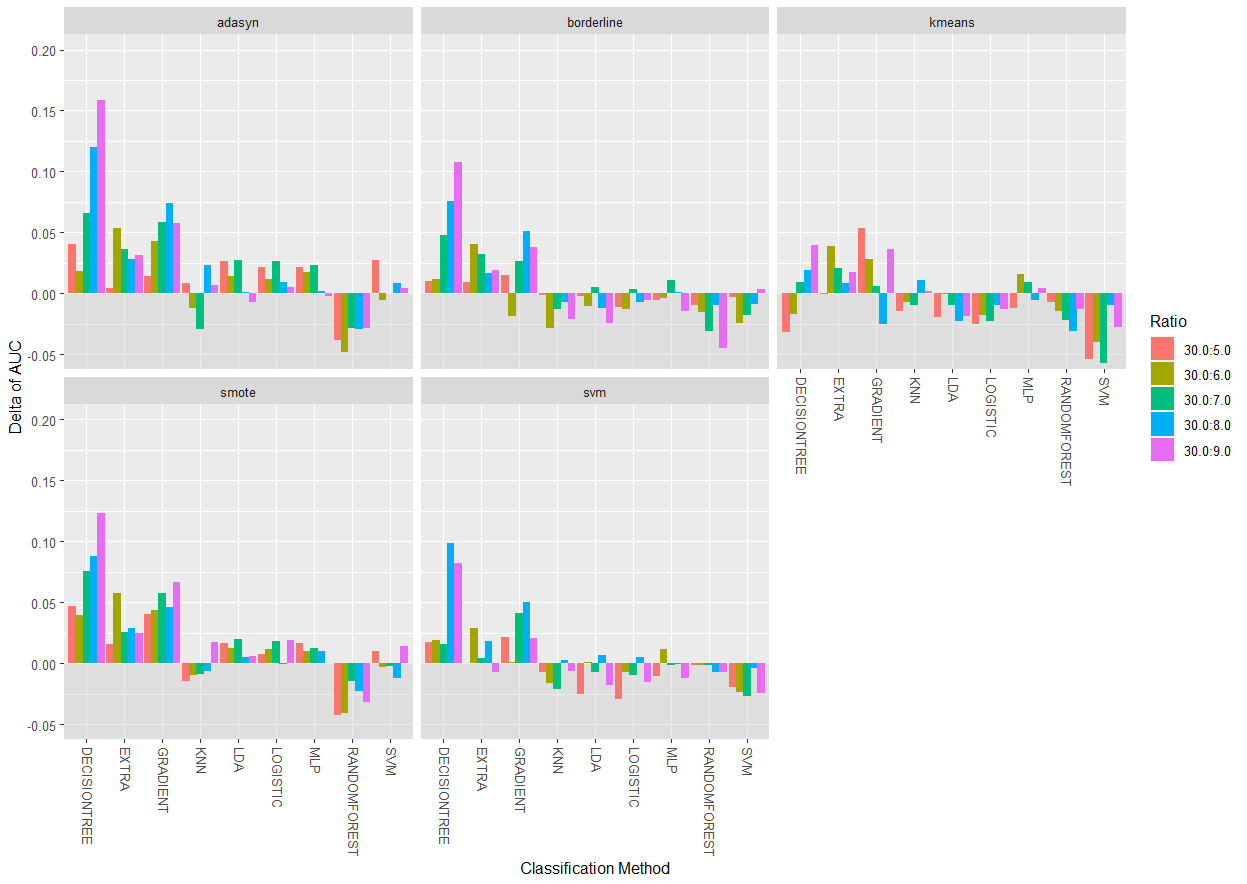
\includegraphics[width=0.9\linewidth]{./figures/imbalance.png}
	\caption[Class imbalance correction techniques]{The impact on F1 scores of class imbalance correction techniques for various ratios and classification strategies can be seen in this visualization. The F1 score of the multi-layer perceptron classification, for instance, starting with a dataset with a 30:2 imbalance, is increased by 85\% when the imbalance is corrected using the ADASYN algorithm. This dataset was first manipulated to achieve the desired ratio before the algorithms were applied. That is, to achieve a 30:1 imbalance, rows in the minority class were randomly dropped.}
	\label{fig:imbalance}
\end{figure}

While the difference in the F1 score achieved with classification using MLP stands out, almost all classification techniques were improved by the correction with one exception. Classification using Random Forest with a dataset with a 30:5 (6:1) imbalance and subsequently corrected to 1:1 using a kMeans approach showed a worse F1 score after correction than before.



\newpage
\section{References}
\printbibliography[heading=none]

%\cite{Wirth2004-li}
\end{document}

